\documentclass[pldi]{sigplanconf-pldi15}

\usepackage{url}                  % format URLs
\usepackage{listings}          % format code
\usepackage{hyperref}
%\usepackage[colorlinks=true,allcolors=purple,breaklinks,draft=false]{hyperref}   % hyperlinks, including DOIs and URLs in bibliography
% known bug: http://tex.stackexchange.com/questions/1522/pdfendlink-ended-up-in-different-nesting-level-than-pdfstartlink
\newcommand{\doi}[1]{doi:~\href{http://dx.doi.org/#1}{\Hurl{#1}}}   % print a hyperlinked DOI
\usepackage{amssymb}
%\usepackage{todonotes}
\usepackage{graphicx}

\newcommand{\TODO}[1]{[\textsl{#1}]}
\newcommand{\code}[1]{\texttt{#1}}
\newcommand{\package}[1]{\code{#1}\cite{#1}}



\begin{document}

\lstset{basicstyle=\footnotesize\ttfamily,mathescape=true,basewidth=0.5em}

\conferenceinfo{PLDI '15}{June 12---20, 2015, Portland, OR, USA.}
\copyrightyear{2015}
%\copyrightdata{}

%\titlebanner{banner above paper title}        % These are ignored unless
\preprintfooter{DRAFT - do not distribute}   % 'preprint' option specified.

\title{Multiple Dispatch for Technical Computing}
%\subtitle{Subtitle Text, if any}

%\authorinfo{Jeff Bezanson \and Jake Bolewski \and Jiahao Chen \and Stefan Karpinski \and Jean Yang \and Alan Edelman}
%	{Massachusetts Institute of Technology}
%	{bezanson@mit.edu, jake.bolewski@gmail.com, jiahao@mit.edu, stefan@karpinski.org, jeanyang@mit.edu, edelman@mit.edu}

\maketitle

\begin{abstract}
  Technical computing (generally, programming for applied math and the sciences) tends
  to be a difficult application area for programming languages to address. This is
  evinced by the unusually large number of specialized languages in the area
  (e.g. MATLAB~\cite{matlab}, R~\cite{rlang}), and the complexity of common
  software stacks, often involving multiple languages and custom code generators.
  We believe this is ultimately due to key characteristics of the domain:
  highly complex operators, a need for extensive code specialization for
  performance, and a desire for permissive high-level programming models that
  support experimentation.
  The Julia language attempts to provide a more effective structure
  for this kind of programming, by employing dynamic multiple dispatch over
  parametric types. The forms of extension and reuse
  permitted by this style are especially valuable for technical computing.
  Here we report on how this paradigm can and has been used to
  express abstractions useful to domain experts, while also providing
  a natural path to better performance for high-level technical code.
\end{abstract}

\category{D.3.3}{PROGRAMMING LANGUAGES}{Language Constructs and Features}

\terms Languages, Multiple dispatch, Multimethods

%\keywords
%Language design, run-time system

\section{Dynamic languages are useful for technical computing}

Engineers, mathematicians and scientists routinely write software for
computational simulations and data analysis to discover new insights.
Users writing code for the purposes of discovery often by definition do not
know what computations they need upfront, but rather discover what they want by
iterating through several different prototypes. Consequently, technical
computing code is often the product of an organic process of continuous
experimentation.

Statically-typed languages focus on proving properties of programs, and constrain
the set of allowed programs in order to do so~\cite{Pierce2002}.
These restrictions can occasionally collide with the way the user would
prefer to think about a problem. In fact this is especially likely to happen
when an answer can be justified mathematically or by specialized domain
knowledge in a way not anticipated by the type system.
In contrast,
dynamic languages embody a realist philosophy: programs are not checked for
correctness, but are executed until termination or when a runtime error is
thrown. The focus is to make sense out of whatever program a user may write.

In other words, a scientist will often run a program in order to find out what
it does---\emph{proving} anything about what it does would be premature, and an
unwelcome distraction. As a result, dynamic languages like
MATLAB~\cite{matlab}, Python~\cite{pythonlib,pythonref} and R~\cite{rlang} have
become popular among technical computing users.

Code written in these languages is difficult to execute efficiently;
the dynamic nature of these languages poses significant challenges for
implementers~\cite{Joisha2001,Joisha2006,Seljebotn2009}. While it is possible
to greatly accelerate dynamic languages with various techniques, for
technical computing the problem does not quite stop there. These systems
crucially depend on large libraries of low-level code that provide array
computing kernels (e.g. matrix multiply). Developing these libraries is a
significant challenge, requiring a range of techniques including templates,
code generation, and manual code specialization.

Julia~\footnote{Julia is free and open--source software available from
\url{http://julialang.org} under the MIT license. In this paper, we describe
the behavior of the v0.3.2 point release.} is a dynamic language designed to
make it easier to express and organize this kind of functionality, while
attempting to maintain the ease-of-use of existing high-level
languages~\cite{Bezanson2012,Bezanson2014b}.

The language is built on polymorphic data and code:

\begin{itemize}
	\item A type system featuring subtyping and parametric types, and
	\item A generic function system with dynamic multiple dispatch
\end{itemize}
%
%% which together naturally express the polymorphism inherent in technical
%% computing. Julia's implementation also features a just-in-time compiler which
%% performs extensive static optimizations such as:

%% \begin{itemize}
%% 	\item Automatic type inference, which minimizes the overhead of dynamic
%% 	      multiple dispatch and largely eliminates the need for explicit
%% 	      type annotations in function bodies.
%% 	\item Tuple elimination
%% 	\item Function inlining
%% 	\item A raft of compiler optimizations such as dead code elimination that
%% 	      are provided by the LLVM library~\cite{Lattner2004}.
%% \end{itemize}

%% This paper aims to explain how Julia's language constructs and compiler
%% optimizations conspire to provide expressiveness without compromising
%% performance, by carefully designing a language that is purposely amenable to
%% static analysis. When combined with an extensive base library for parallel
%% execution and numerical analysis, Julia provides a convenient environment for
%% rapid prototyping of new analytics which can also be deployed performantly,
%% often within a factor of two of the speed of native, hand-written C code.

While multiple dispatch has been extensively studied as an object-oriented
paradigm in the past, it has not been widely adopted in practice~\cite{Muschevici:2008}.
However in Julia, a growing number of scientific programmers are using it
extensively---we might even say gleefully. The key property of multiple
dispatch for this domain seems to be that it allows programs (particularly libraries)
to be written incrementally, in small pieces, where each piece has a method signature
specifying \emph{declaratively} how it fits into the whole.
More sophisticated types make this process work better, since they allow new
definitions to be added in more situations.


\section{Type system}

Julia is a dynamic language, i.e.\ it has no static semantics. As such, Julia
does not have types in the strict sense, but rather run-time type tags used to
describe and differentiate objects~\cite[Section 11.10, p. 142]{Pierce2002}.
We tend to use the term ``type'' anyway, as programmers seem to be familiar
with this use of it~\cite{Tratt2009,Kell2014}.

All values in a dynamically typed language have two semantic components:
a \emph{tag} and some \emph{data}. The tag classifies the data, which are the
contents of some block of memory whose format is set by the programming
language. Tags are useful for both users and compilers for deciding what to do
to values, but incur overhead which increases the memory footprint of a data
item. This overhead motivates most dynamically typed languages to simplify and
minimize their tag systems.

Julia instead allows type tags with nested structure, indeed forming nearly
arbitrary symbolic expressions. This has two immediate benefits: first,
it expands the criteria programmers have available for dispatching, and second,
provides more information to the compiler. Julia's type tags are designed
to form a lattice structure, which enables effective dataflow analysis.
In general, Julia's types allow programs to reason about:

\begin{itemize}
\item when code is applicable (dispatch),
\item what to specialize on,
\item memory layout, and
\item what can be statically known about a potential value.
\end{itemize}
%
Furthermore, types are first-class values, allowing programs that can compute
on types and reason about all of the above.


\subsection{Kinds of types}

Julia has different kinds of types which can be formally summarized as:

\begin{lstlisting}
Type ::= Abstract | Data | Tuple | Union | UnionAll
Tag ::= Data | Tuple

Data ::= Name (Type...) Abstract } invariant, nominative
Abstract ::= Name (Type...) Abstract }
Tuple ::= (Type$_1$, Type$_2$...) |
          (Type$_1$, Type$_2$, ..., Type$_n$) } covariant
Union ::= Union(Type$_1$, Type$_2$, ...)
UnionAll ::= UnionAll T<:Type . Type
\end{lstlisting}

\begin{description}

\item[Data types] are types with associated constructors. They
	are further subdivided into:
	\begin{description}
	
	\item[Bits types] like double precision floating point numbers
	(\verb|Float64|) and 32-bit signed integers (\verb|Int32|), which can
	be stored unboxed as raw bits without tag overhead,

	\item[Abstract data types] which have an internal representation
		declared with the \verb|type| keyword, and
		
	\item[Immutable types] which are similar to abstract data types
		declared with the \verb|immutable| keyword, but whose internal
		variables are immutable, thus potentially allowing for unboxed
		representations.

	\end{description}

\item[Abstract types] define an uninstantiable type with no declared
	representation. They are used as declared supertypes of leaf types
	(which are concrete and instantiable).

\item[Tuple types] \code{(T1, T2,...)} which are constructed from the Cartesian
	product of zero or more existing types \code{T1}, \code{T2},
	etc.~\cite[Sec. 11.7]{Pierce2002} Tuples are covariant. They may also
        end with \code{...}, matching any number of trailing elements.

\item[Union types] written as \code{Union(T1, T2,...)} are the join of zero,
	or two or more, types \code{T1}, \code{T2}, ...~\cite[Sec.
	15.7]{Pierce2002}
	%
	\begin{equation}
		\texttt{Union}(T_1, T_2, ..., T_N) = \bigvee_{i=1}^N T_i 
	\end{equation}
	%
	The union with zero types, \code{Union()}, is simply the bottom type.
	%
	%% Julia's \code{Union}s are untagged and disjoint, which allows for some
	%% simplifications in their construction:
	%% \begin{itemize}
	%% 	\item If there are types \code{S} and \code{T} obeying the
	%% 		subtyping relation \code{S <: T} in the union
	%% 		constructor, then \code{S} is deleted ($\beta$-reduced)
	%% 		from the final union type constructed. This
	%% 		simplification includes the special case where \code{S}
	%% 		and \code T are identical.

	%% 	\item A union type \code{Union(T)} with a single type parameter
	%% 		\code{T} is identical (by $\eta$-reduction) to just
	%% 		\code{T}.
	%%\end{itemize}

\item[UnionAll types] which are type unions that are implicitly quantified over
	all types \verb|S| satisfying a subtype relation \verb|S <: T|.

\end{description}

\verb|Abstract| and \verb|Data| types have two additional features:

\begin{enumerate}
	\item They each have one declared supertype, allowing for subtype
	relations to be defined as described in Section~\ref{sec:subtyping}.

	\item They can be defined with zero or more types as parameters as
	described in Section~\ref{sec:typeparameters}.
\end{enumerate}

%% Type parameters and subtyping, when combined with late binding semantics
%% associated with dynamic dispatch, provides Julia with rich polymorphic
%% expressiveness, facilitating code reuse and an incremental style of
%% programming~\cite{Castagna1997} that is well--suited to the rapid prototyping
%% of technical codes.

\subsection{Subtyping}
\label{sec:subtyping}

Julia requires \verb|Abstract| and \verb|Data| types to have exactly one
declared supertype (defaulting to $\top$ if not explicitly declared).
We conjecture that the subtype relation \verb|<:| is well-defined and
decidable, and that types are closed under meet ($\wedge$) and
join ($\vee$).

%% The notion of subtyping is analogous to subset relations, but the subset
%% relation is not just over sets of permitted values, but also the interface,
%% i.e.\ set of functions allowed to compute over the types being
%% compares~\cite{Scott1976,Liskov1974,Liskov1994}. Furthermore, a mathematical
%% quantity can have more than one encoding as a compiler value. For example, each
%% integer in the set {0, 1, \dots, 255} has a 1:1 correspondence with an 8-bit
%% unsigned integer (\verb|Uint8|), and also a 1:1 correspondence as a
%% double-precision floating point number (\verb|Float64|). Nevertheless,
%% \verb|Uint8| is \textit{not} a subtype of \verb|Float64| since not all
%% operations on the former behave identically to operations on the latter. One
%% example is subtraction, which returns different values for the different types:

%% \begin{lstlisting}
%% julia> uint(5)-uint(253)
%% 0xffffffffffffff08

%% julia> 5.0 - 253.0
%% -248.0
%% \end{lstlisting}
%% %
%% In contrast, \verb|Union(Uint8, Float64)| is a subtype of \verb|Real| by
%% transitivity of the declared supertype relations, which allow \verb|Real|
%% to abstractly represent disjoint sets of values and their interfaces.


\subsection{Type parameters}
\label{sec:typeparameters}

\verb|Abstract| and \verb|Data| types can take one or more parameters. These
types are superficially quite similar to parametric types in existing
languages, but are actually intended simply for expressing information, rather
than implementing the formal theory of parametric polymorphism.

The following example, from Julia's standard library, describes a \verb|SubArray|
type that provides an indexed ``view'' into another array. It begins by
defining a \verb|Union| of what kinds of indexes may be used, then uses this
definition to define indexed views:

\begin{lstlisting}
  typealias RangeIndex Union(Int,Range{Int},UnitRange{Int})

  type SubArray{T, N,
		A<:AbstractArray,
		I<:(RangeIndex...,)} <: AbstractArray{T,N}
      # definition body omitted
  end
\end{lstlisting}
%
\verb|SubArray| has parameters \verb|T| for an element type, \verb|N| for the
number of dimensions, \verb|A| for the underlying array type, and \verb|I|
for the tuple of indexes that describe which part of the underlying array
is viewed. The \verb|<:| declares \verb|SubArray| to be a subtype of
\verb|AbstractArray|.

An unusual feature of this system is that it tries to hide type kinds from
the user. The identifier \verb|SubArray| by itself does not refer to a
type constructor that must be instantiated. Rather it is itself a type
that functions as the supertype of all \verb|SubArray|s. This allows
convenient shorthand for writing methods that are agnostic about type parameters.
It also makes it possible to add more type parameters in the future, without
necessarily updating all client code.

When implementing \verb|SubArray| and client code using it, it is useful
to be able to dispatch on all of these parameters. For example, when
\verb|I| matches \verb|(UnitRange, RangeIndex...)| then the \verb|SubArray|
is contiguous in the leading dimension, and more efficient algorithms can
generally be used. Or, linear algebra code might want to restrict the
number of dimensions \verb|N| to 1 or 2.

\subsubsection{Variance}

The subtyping rules for parametric types require reasoning about variance,
i.e.\ the relation between subtype relations of the parametric types and
subtype relations of the parameters. The conventional wisdom is that type
safety allows covariance if components are read but not written, and
contravariance if they are written but not read~\cite{Castagna1995}. As type
parameters can represent the types of mutable fields in a \verb|type| which can
be read or written, then the only safe choice is invariance. Thus Julia's
parametric types are invariant.

Parametric invariance has some subtle consequences for Julia's type system.
First, parametric types introduce many short, finite length chains into the
type lattice. Consider the very simple type system of
Figure~\ref{fig:lattice}a, with two leaf (instantiable types) types \textbf{1}
and \textbf{2} representing singleton values 1 and 2 of the natural numbers,
\verb|Nat|. A user can augment the lattice with a new parametric type
\verb|S{T}|. If there is no restriction whatsoever on the type parameter
\verb|T|, then there are 5 different parametric types of the form \verb|S{T}|.
Furthermore, each \verb|S{T}| has supertype \verb|S| by construction, and by
invariance of \verb|T| there are no values of the type parameters \verb|T| and
\verb|U| such that \verb|S{T}| is a subtype of \verb|S{U}|. Additionally, none
of the types \verb|S{T}| is a subtype or supertype of any of \textbf{1},
\textbf{2} or \verb|Nat|. Thus each \verb|S{T}| appears in exactly one finite
poset $\bot$ \verb|<: S{T} <: S <:| $\top$, and the new type lattice has the
structure shown in Figure~\ref{fig:lattice}b. Note that \verb|S{|$\top$\verb|}|
is a concrete type with type parameter $\top$ (\verb|Any|), while \verb|S{T}|
is a synonym for the abstract type \verb|S| where \verb|T| is a \verb|TypeVar|
with lower bound $\bot$ and upper bound $\top$. 

\begin{figure}
	\centering
	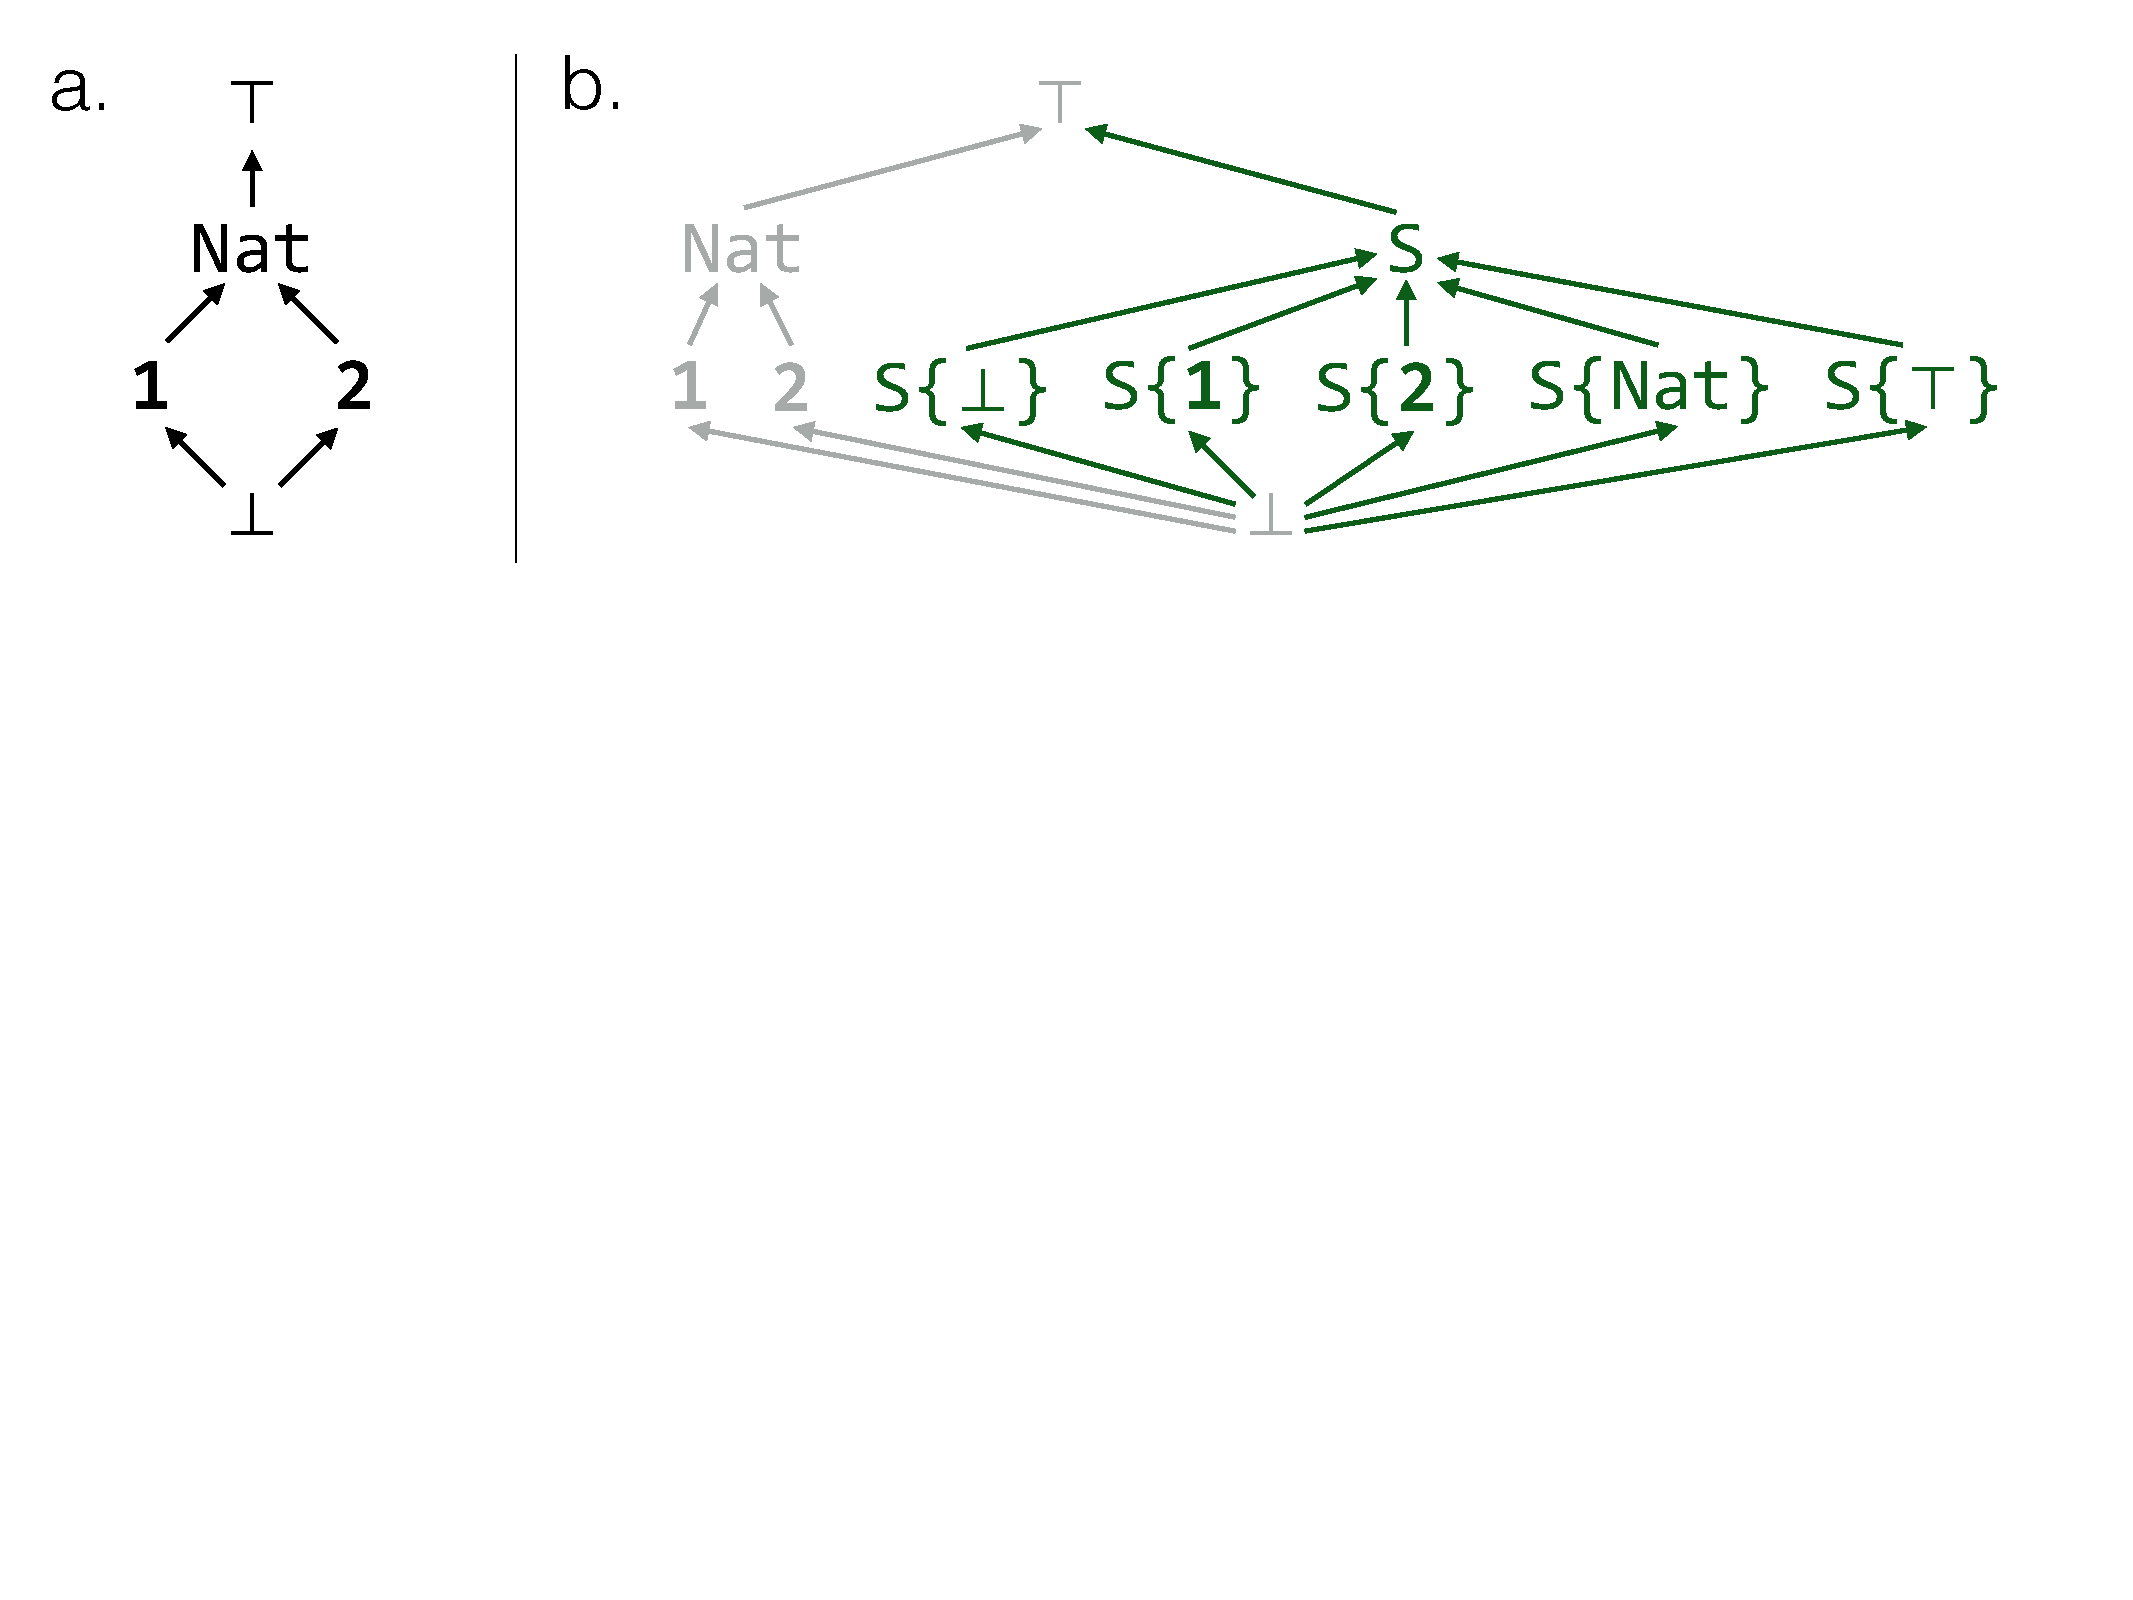
\includegraphics[width=\columnwidth]{fig-lattice}
	\caption{
		\textbf{a.} A simple lattice with bottom type $\bot$, top type
		$\top$, singleton types \textbf{1} and \textbf{2}, and their
		supertype \texttt{Nat}.
		\textbf{b.} The same lattice extended with a parametric type
		\texttt{S\{T\}} with no restriction on the type parameter
		\texttt{T}, showing that for each \texttt{T}, invariance
		requires that the corresponding type \texttt{S\{T\}} be a leaf
		type (i.e.\ instantiable), even if \texttt{T} itself is not a
		leaf type.}
	\label{fig:lattice}
\end{figure}

Second, the example of Figure~\ref{fig:lattice} illustrates how invariance of
type parameters requires parametric types to be instantiable with any type
parameter, regardless of whether the parameter corresponds to an abstract or
concrete type. The rationale for this behavior allows for the Julia compiler to
reason about different representations, and is perhaps best explained in the
context of arrays. For arrays, the type parameter describes the set of possible
element types ~\cite{Bezanson2014}, so an \verb|Array{Float64}|
can only contain concrete elements of type \verb|Float64|, whereas an
\verb|Array{Real}| can contain elements that are subtypes of \verb|Real| such
as \verb|Int|, \verb|Float64| or even \verb|Rational|. The former array
consists of concrete immutable elements and can be reified with a single
pointer to a contiguous memory block with the tags for each element elided,
resulting in a memory layout which can interoperate with C or Fortran code as
native array data structures. The latter array can store more diverse objects,
but the element type provides no information about the mutability of each
element. Consequently, the array must be represented in memory with pointers to
boxed elements, so that checks from generated LLVM code can be inserted that
call back into the Julia runtime to determine the actual type of the stored
element at run--time. Thus describing arrays as parametric types allows
different data structures to be used under the hood without any semantic
changes imposed on users, thus allowing for more performance in one case and
greater flexibility in the other.

Subtyping and type parameters combine to provide powerful expressions of
polymorphism, similar to those formalized by $\lambda$--calculi such as
System~F$_\le$~\cite{Cardelli1985}. However, the interaction of these two
Julia languages features can be subtle and confusing. For example, \verb|Real|
is not a subtype of \verb|Complex| because for each type \verb|T| that is a
subtype of \verb|Real|, there is a corresponding instantiable type
\verb|Complex{T}|. None of these correspond to \verb|Real| since there is no
\verb|T| such that \verb|Complex{T}| is a one-component number, and each
concrete type only has $\bot$ as its subtype.

Another more subtle situation arises from parametric invariance: each value of
\verb|Complex{Int64}| is a Gaussian integer, i.e., a complex number where each
component is an integer, and so each \verb|Complex{Int64}| is in 1:1
correspondence with a value in \verb|Complex{Integer}| and also in
\verb|Complex{Real}|. Nevertheless, \verb|Complex{Int64}| is a subtype of
neither \verb|Complex{Integer}| nor \verb|Complex{Real}| due to parametric
invariance. However, all of these are subtypes of \verb|Complex|.

%% The instantiability of parametric types with non-leaf type parameters can lead
%% to subtle performance bottlenecks and reasoning pitfalls. Consider the three
%% \code{Complex} numbers

%% \begin{lstlisting}
%% z1 = Complex{Float64}(0.0, 1.0)
%% z2 = Complex{FloatingPoint}(0.0, 1.0)
%% z3 = Complex{Union(Rational, Integer, Float64)}(0, 1.0)
%% \end{lstlisting}
%% %
%% which are all numerically equivalent (i.e.\ \verb|z1 == z2 == z3|), but not
%% identical in the \textit{egal} sense~\cite{Baker1993} (\verb|===| in Julia).
%% If we inspect the variables using Julia's \verb|dump| command, we get:

%% \begin{lstlisting}
%% julia> dump(z1)
%% Complex{Float64}
%%   re: Float64 0.0
%%   im: Float64 1.0

%% julia> dump(z2)
%% Complex{FloatingPoint}
%%   re: Float64 0.0
%%   im: Float64 1.0

%% julia> dump(z3)
%% Complex{Union(Integer,Float64,Rational{T<:Integer})}
%%   re: Int64 0
%%   im: Float64 1.0
%% \end{lstlisting}
%% %
%% We see that the \verb|::T| tag annotation on a field does not guarantee that
%% the type of a value placed in the field in any given instance of that type is
%% exactly of type \verb|T|, merely that it is a subtype of \verb|T|. Only for
%% \verb|z1| can the compiler elide the run--time type checks and hence represent
%% \verb|z1| with the fields contiguous in memory without indirection, which
%% increases the performance of code working on \verb|z1| relative to \verb|z2|
%% and \verb|z3|. Nevertheless, all three are fully--fledged \verb|Complex|
%% numbers and support all the semantics associated with the \verb|Complex| type.
%% In this way, Julia allows for a meaningful compromise being flexibility and
%% performance.


\subsection{Type conversion}

While Julia code can be written without
explicitly reasoning about types, the ability to do so is sometimes necessary for
understanding code performance issues. Julia provides the \verb|convert(T, x)|
function which converts a value \verb|x| to its corresponding representation in
the type \verb|T|. This is a generic function like any other, but since
\verb|T| is typically a compile-time constant this can serve as a mechanism for
limiting polymorphism in codes where performance considerations are important.

Notice that the idea of converting a value of type \verb|A| to type \verb|B|
does not naturally belong to one type or the other, which favors multiple
dispatch over classes. Conversion also benefits from open extension:
mathematical objects often have embeddings in multiple domains, not all of
which might be known or desired by the original author of some code. For
example numbers can be embedded in matrices as diagonal matrices, but not
all users are likely to find this correspondence helpful.


\section{Generic functions and multimethods}

Mathematical thought is
naturally polymorphic. Multimethods are a natural mechanism for capturing such
polymorphism~\cite{Bezanson2014b,Chen2014}. Consider an operation as
fundamental as multiplication: an expression like \verb|a*b| can mean:

\begin{itemize}
	\item a matrix--matrix product,
	\item a matrix--vector product, or
	\item a scalar--vector product,
\end{itemize}
%
to name just a few possibilities. A generic function system supporting
multimethods allows for the \verb|*| function to be polymorphic, expressing a
common metaphor for different kinds of multiplication which can be
disambiguated by the types of \verb|a| and \verb|b|. In contrast, languages
supporting only classes cannot capture the full extent of polymorphism in
\verb|*| in method dispatch: as classes inherently support only single dispatch
on the first argument, each method \verb|*| defined for each class \verb|a|
must contain different code blocks for each possible type of \verb|b|, thus in
practice requiring multiple dispatch to be emulated using virtual methods and
visitor patterns~\cite{designpatterns}. Furthermore, implementing binary methods can
require knowing the internal representation of both objects \verb|a| and
\verb|b|, especially for performance reasons~\cite{Bruce1995}. Such knowledge
fundamentally corrupts the abstraction of class-based encapsulation, as the
methods associated with \verb|a| must know implementation details of all
possible objects \verb|b| that \verb|a| may interact with.
In contrast, there is no abstraction leak associated with allowing a generic
function \verb|*| knowledge about the internal representations of the types it
works on.

Multiplication represented by \verb|*| can be extended, for
example, to multiplication between quaternions, or even to $N$--ary
matrix-matrix products, where associativity\footnote{Neglecting the lack of
exact associativity in some fields such as floating-point numbers.} allows
matrix-matrix products to be regrouped so as to minimize the total memory
footprint and operation count~\cite{Hu1984}.

The extensibility of Julia's generic functions and types allow users to
define new behaviors that intermix new types and new functions. The price we pay
for such flexibility, of course, is that dynamic function dispatch incurs
greater overhead: unlike in a single dispatch language, multiple lookups in
method tables may be necessary to determine which method is most
appropriate~\cite{Bruce1995}. Type inference is
useful for minimizing or even eliminating the
overhead associated with multiple dispatch.

Another, subtler point is that unlike other object models, generic functions
provide no encapsulation guarantees, since they are allowed to peer into the
internal representation of types. Consequently, type safety requires stringent
criteria on the allowed variances of types~\cite{Allen2011}.


%% NOTE: This section is actually very good but I don't think we can use it unless
%% we show what this feature is good for. Jiahao has said he doesn't feel this is
%% all that useful for technical computing, so better to leave it out.

%% \subsection{Diagonal dispatch}

%% Diagonal dispatch is a special refinement of method dispatch that occurs when a
%% type parameter appears in more than position in the method signature, e.g.:

%% \begin{lstlisting}
%% f{T}(x::T, y::T)
%% \end{lstlisting}
%% %
%% Diagonal dispatch occurs only for concrete types \verb|T|. For example,
%% \verb|f(1, 2)| works as the arguments are of type \verb|(Int, Int)|, but not
%% \verb|f(1, 2.0)| as the arguments are of type \verb|(Int, Float64)|, even
%% though that tuple type is a subtype of \verb|(T, T)| where
%% \verb|T = Union(Int,| \verb|Float64)| or any larger common supertype of \verb|Int| and
%% \verb|Float64|. Thus for diagonal dispatch to match only concrete \verb|T|s,
%% the tuple of arguments is treated \textit{not} covariantly, but rather,
%% \textit{invariantly}. Although this is an unusual special--casing of tuple
%% behavior, the greater specificity allowed by invariance makes diagonal dispatch
%% more useful in practice by matching only concrete types, particularly when
%% \verb|T| appears multiple times in the method signature, e.g.\ 
%% \verb|f{T}(x::T, y::T, z::T)| or even \verb|f{T}(xs::T...)|. 

%% The \textit{diagonal} nature of diagonal dispatch is apparent when considering
%% the dispatch table for the method \verb|f{T}| \verb|(x::T, y::T)|: when written
%% out as a table with all possible types of \texttt{x} and \texttt{y} along the
%% rows and columns as shown in Table~\ref{tab:diagonal}, the method dispatches
%% only along the diagonal of the table.

%% \begin{table}
%% \begin{tabular}{c | c c c c c}
%% 	& \verb|Int| & \verb|Float64| & \verb|Bool| & \verb|Real| & $\cdots$ \\ \hline
%% 	\verb|Int|     & \checkmark &  &  &  & \\
%% 	\verb|Float64| &  & \checkmark &  &  & \\
%% 	\verb|Bool|    &  &  & \checkmark &  & \\
%% 	\verb|Real|    &  &  &  &  & \\
%% 	$\vdots$       &  &  &  &  &
%% \end{tabular}
%% \caption{Dispatch table for the function \texttt{f} with method
%% \texttt{f\{T\}(x::T, y::T)}, showing that dispatch occurs only along the
%% diagonal with all possible types of \texttt{x} and \texttt{y} along the rows
%% and columns.}
%% \label{tab:diagonal}
%% \end{table}


\section{Type inference}
\label{sec:inference}

It is well known that type inference can be used to move tag manipulations
and method lookup to compile time, thus eliminating most overhead from
the execution of dynamically-typed code~\cite{Kaplan1977,Kaplan1980}.
Data flow type inference~\cite{Nielson2005,Khedker2009}
is especially useful in this context, as its
flow-sensitivity yields good type information even if the type of a program
variable is different at different points in the code.
Data flow analysis, particularly in the
forward direction, captures the human intuition of how programs work:
values start at the top and move through the program step by step.
Another advantage of this approach is that it is \emph{not} speculative:
it yields correct deductions about types that, in the best case, allow
overhead to be removed entirely. This property is important to technical
users, who need languages that can match the performance of C and Fortran.

Unfortunately data flow type inference is relatively easily defeated
by dynamic language programs that are too ``type complex''. If the library
functions used might return too many different types, or there are too
many paths through user code, the resulting type information might not
be useful.

Julia's design was intended to help mitigate this problem. By encouraging
code to be written in small pieces labeled with type information (for
dispatch), it is easier for the compiler to rule out execution paths
that do not actually occur.

Type inference in Julia occurs after code is parsed, macro--expanded, and
lowered into a static single assignment (SSA) intermediate representation
(IR)~\cite{Alpern1988,Rosen1988} that facilitates data flow
analysis~\cite{Cousot1977,Cousot2000,Nielson2005} and is relatively
straightforward to map onto LLVM IR~\cite{Lattner2004}. Julia uses Mohnen's algorithm
for abstract interpretation~\cite{Cousot1992} which works directly on the SSA
IR~\cite{Mohnen2002}. The abstract semantics are described internally using
transfer functions (a.k.a.\ t--functions or flow functions), which approximate
program semantics by inferring possible output types based on the types of
the inputs.

In practice, the expressiveness of Julia's late binding semantics, combined
with the presence of potentially infinite types such as varargs tuples
\verb|(T...)|, complicate type inference.
%The combination of late binding and
%the ability to use generic functions as type parameters also means that the
%general type inference problem is undecidable, as was proved for the System F
%calculus~\cite{Wells1999}.
Therefore practical type inference necessitates
widening heuristics, which reduce computational costs and guarantee termination
in the presence of recursive types~\cite{Cousot1992a}. Examples of such
heuristics include widening (pessimizing) type unions and tuple types which
exceed a certain length, and limiting the maximal depths of types
and tuples analyzed.
%Widening operations are not guaranteed to be monotonic,
%i.e.\ the ordering of approximations may no longer be preserved, and hence the
%fixed point computed by abstract interpretation is not guaranteed to be
%minimal even in a formally monotonic data flow framework~\cite{Cousot1992}.
%Thus the inferred types are not necessarily the least upper bounds on the
%possible values~\cite{Kaplan1977,Kaplan1980}.

Julia provides language features to help users inspect the results of type
inference and specify additional type information where necessary to sharpen
the types of variables.

\begin{enumerate}

	\item The base library provides introspection functions like
	\verb|code_typed|, which allow users to inspect generated type
	annotations and avoid second--guessing the compiler's intentions.

	\item Variables can also be given explicit \textbf{type annotations};
	changing \verb|x = 0| to \verb|x::Float64 = 0| declares \verb|x| to be
	of type \verb|Float64| within the current scope, and all assignments
	\verb|x = _| implicitly call the type conversion function
	\verb|convert(Float64, _)|.

	\item Expressions can be given \textbf{type assertions}; changing
	\verb|x += y| to \verb|x += y :: Int| asserts that \verb|y| must be of
	type \verb|Int| or otherwise raise a run-time error.

\end{enumerate}
%
External packages like \package{TypeCheck.jl} and \package{Lint.jl} provide
further static analyses which are useful for detecting type-related issues.


\section{Applications in technical computing}

In this section, we describe how the type system, generic functions and type
inference interact in Julia code for scientific computations in base library
code as well as registered packages. 

\subsection{Type promotion}

The type system and generic function system allow for type promotion rules to
be specified in the base library rather than be hard--coded into a given
implementation~\cite{Bezanson2012a}. For example, simple arithmetic functions
on general numeric types in Julia's base library contain methods of the form:

\begin{lstlisting}
+(x::Number, y::Number) = +(promote(x,y)...)
*(x::Number, y::Number) = *(promote(x,y)...)
-(x::Number, y::Number) = -(promote(x,y)...)
/(x::Number, y::Number) = /(promote(x,y)...)
^(x::Number, y::Number) = ^(promote(x,y)...)
\end{lstlisting}

For example, an operation like \verb|2 * 3.4| is evaluated under the hood as
follows:

\begin{lstlisting}
*(2, 3.4) = *(promote(2, 3.4)...)
          = *(convert(promote_type(Int,Float64),2),
	      convert(promote_type(Int,Float64),3.4))
          = *(convert(Float64,2), convert(Float64,3.4))
	  = *(2.0, 3.4)
	  = 6.8
\end{lstlisting}
%
where \verb|promote(x, y)| promotes the values \verb|x| and \verb|y| to
numerically equivalent values of a common supertype, and
\verb|promote_type(S,T)| computes a common supertype of \verb|S| and \verb|T|.
The latter calls a custom promotion rule, if defined, and defaults otherwise to
the join \verb|S|$\vee$\verb|T|.

Type promotion allows for different functions and methods to share a common and
consistent logic for polymorphism. The implementation of type promotion
leverages the type system to allow for greater code reuse across different
methods and functions. Furthermore, it is a part of the Julia language which
can be built entirely from other language constructs.


\subsection{Numerical linear algebra library}

Designing a general-purpose linear algebra library involves several different
layers of complexity, and has been described as implementing the following
meta-program~\cite{Demmel2007}:

{\small
\begin{verbatim}
(1) for all linear algebra problems
    (linear systems, eigenproblems, ...)
(2)  for all matrix types
     (general, symmetric, banded, ...)
(3)   for all data types (real, complex,
      single, double, higher precision)
(4)    for all machine architectures and
       communication topologies
(5)     for all programming interfaces
(6)      provide the best algorithm(s) available
         in terms of performance and accuracy
         (``algorithms'' is plural because
         sometimes no single one is always best)
\end{verbatim}
}
%
The six-tiered hierarchy neatly delineates how the basic collection of linear
algebra problems (1) have to be specialized by data representation (2-3) and
machine details (4), which are then used to decide which specific algorithms
(5-6) to use.

Many systems provide optimized implementations of standard libraries for
numerical linear algebra like BLAS (Basic Linear Algebra Subprograms) and
LAPACK (Linear Algebra PACKage). Computational routines can be customized
for individual microarchitectures and can reach a significant fraction of
theoretical peak FLOPS. However, these libraries inherit archaic Fortran 77
interfaces and hence tend to restrict routine names to six letters or shorter.
When combined with the lack of polymorphism in Fortran, the names are terse and
cryptic to nonexperts: a typical routine like \verb|DSTEV| solves the
eigenvalue problem (\verb|EV|) for symmetric tridiagonal matrices (\verb|ST|)
with double precision floating point entries (\verb|D|), and furthermore takes
eight positional arguments specifying the inputs, outputs, computation mode,
and scratch variables. The lack of polymorphism results in redundancy due to
lack of code reuse, which hinders the implementation of new algorithms (which
have to be reimplemented for each level of floating-point precision) and new
routines for such as mixed-precision and quad precision routines (which must
implement all the existing algorithms).

The code redundancy problem is largely ameliorated with the combination of type
polymorphism and dynamic multiple dispatch. The six-tiered hierarchy above maps
naturally onto different language constructs in Julia as follows:

\vspace{12pt}
\begin{tabular}{c l l}
	\hline
	Tier & Description & Language construct \\ \hline
	1 & linear algebra problems & generic function \\
	2 & matrix types & parametric types \\
	3 & data types & type parameter \\
	4 & machine architectures & method body \\
	5 & programming interfaces & generic function \\
	6 & (poly)algorithms & method body \\ \hline
\end{tabular}
\vspace{12pt}

The generic function system allows for fast specializations and generic
fall-backs to coexist, thus allowing for speed when possible and flexibility
otherwise. For example, Julia provides generic fall-back routines to do matrix
computations over arbitrary fields of element types, providing the ability to
compute on numeric types which are not mappable to hardware floating point
types. This can be useful to perform matrix computations in exact rational
arithmetic or software--emulated higher precision floating point arithmetic to
verify the implementations of algorithms or to detect the possibility of
numerical instability associated with roundoff errors. These general purpose
routines coexist with BLAS and LAPACK wrappers, thus allowing dispatch onto
performant code when available, and general code otherwise. User code can be
written that will work regardless of element type (Tier 3), and can be tuned
for performance later.

\subsection{Dynamic dispatch in matrix functions}

Dynamic, i.e.\ late binding, dispatch allows for high performance
polyalgorithms with specialized code paths depending on matrix properties which
can only be inferred at runtime based on the specific values of the inputs. For
example, the matrix square root (\verb|sqrtm|) has two methods defined:

\begin{itemize}
	\item For symmetric (or Hermitian) matrices, where the answer can be
		computed by diagonalization,
	\item For general dense matrices, where the answer uses the more
		expensive (but also more general) Schur
		factorization~\cite{Higham2008}.
\end{itemize}
%
The latter method contains a run time check for symmetry and dispatches upon
the former if present. Thus as summarized in Figure~\ref{fig:sqrtm}, dynamic
dispatch allows the same performant kernel to be called even in situations
where the user does not know if a particular input matrix is symmetric, or even
that specialized algorithms for symmetric matrices exist.

\begin{figure}
	\centering
	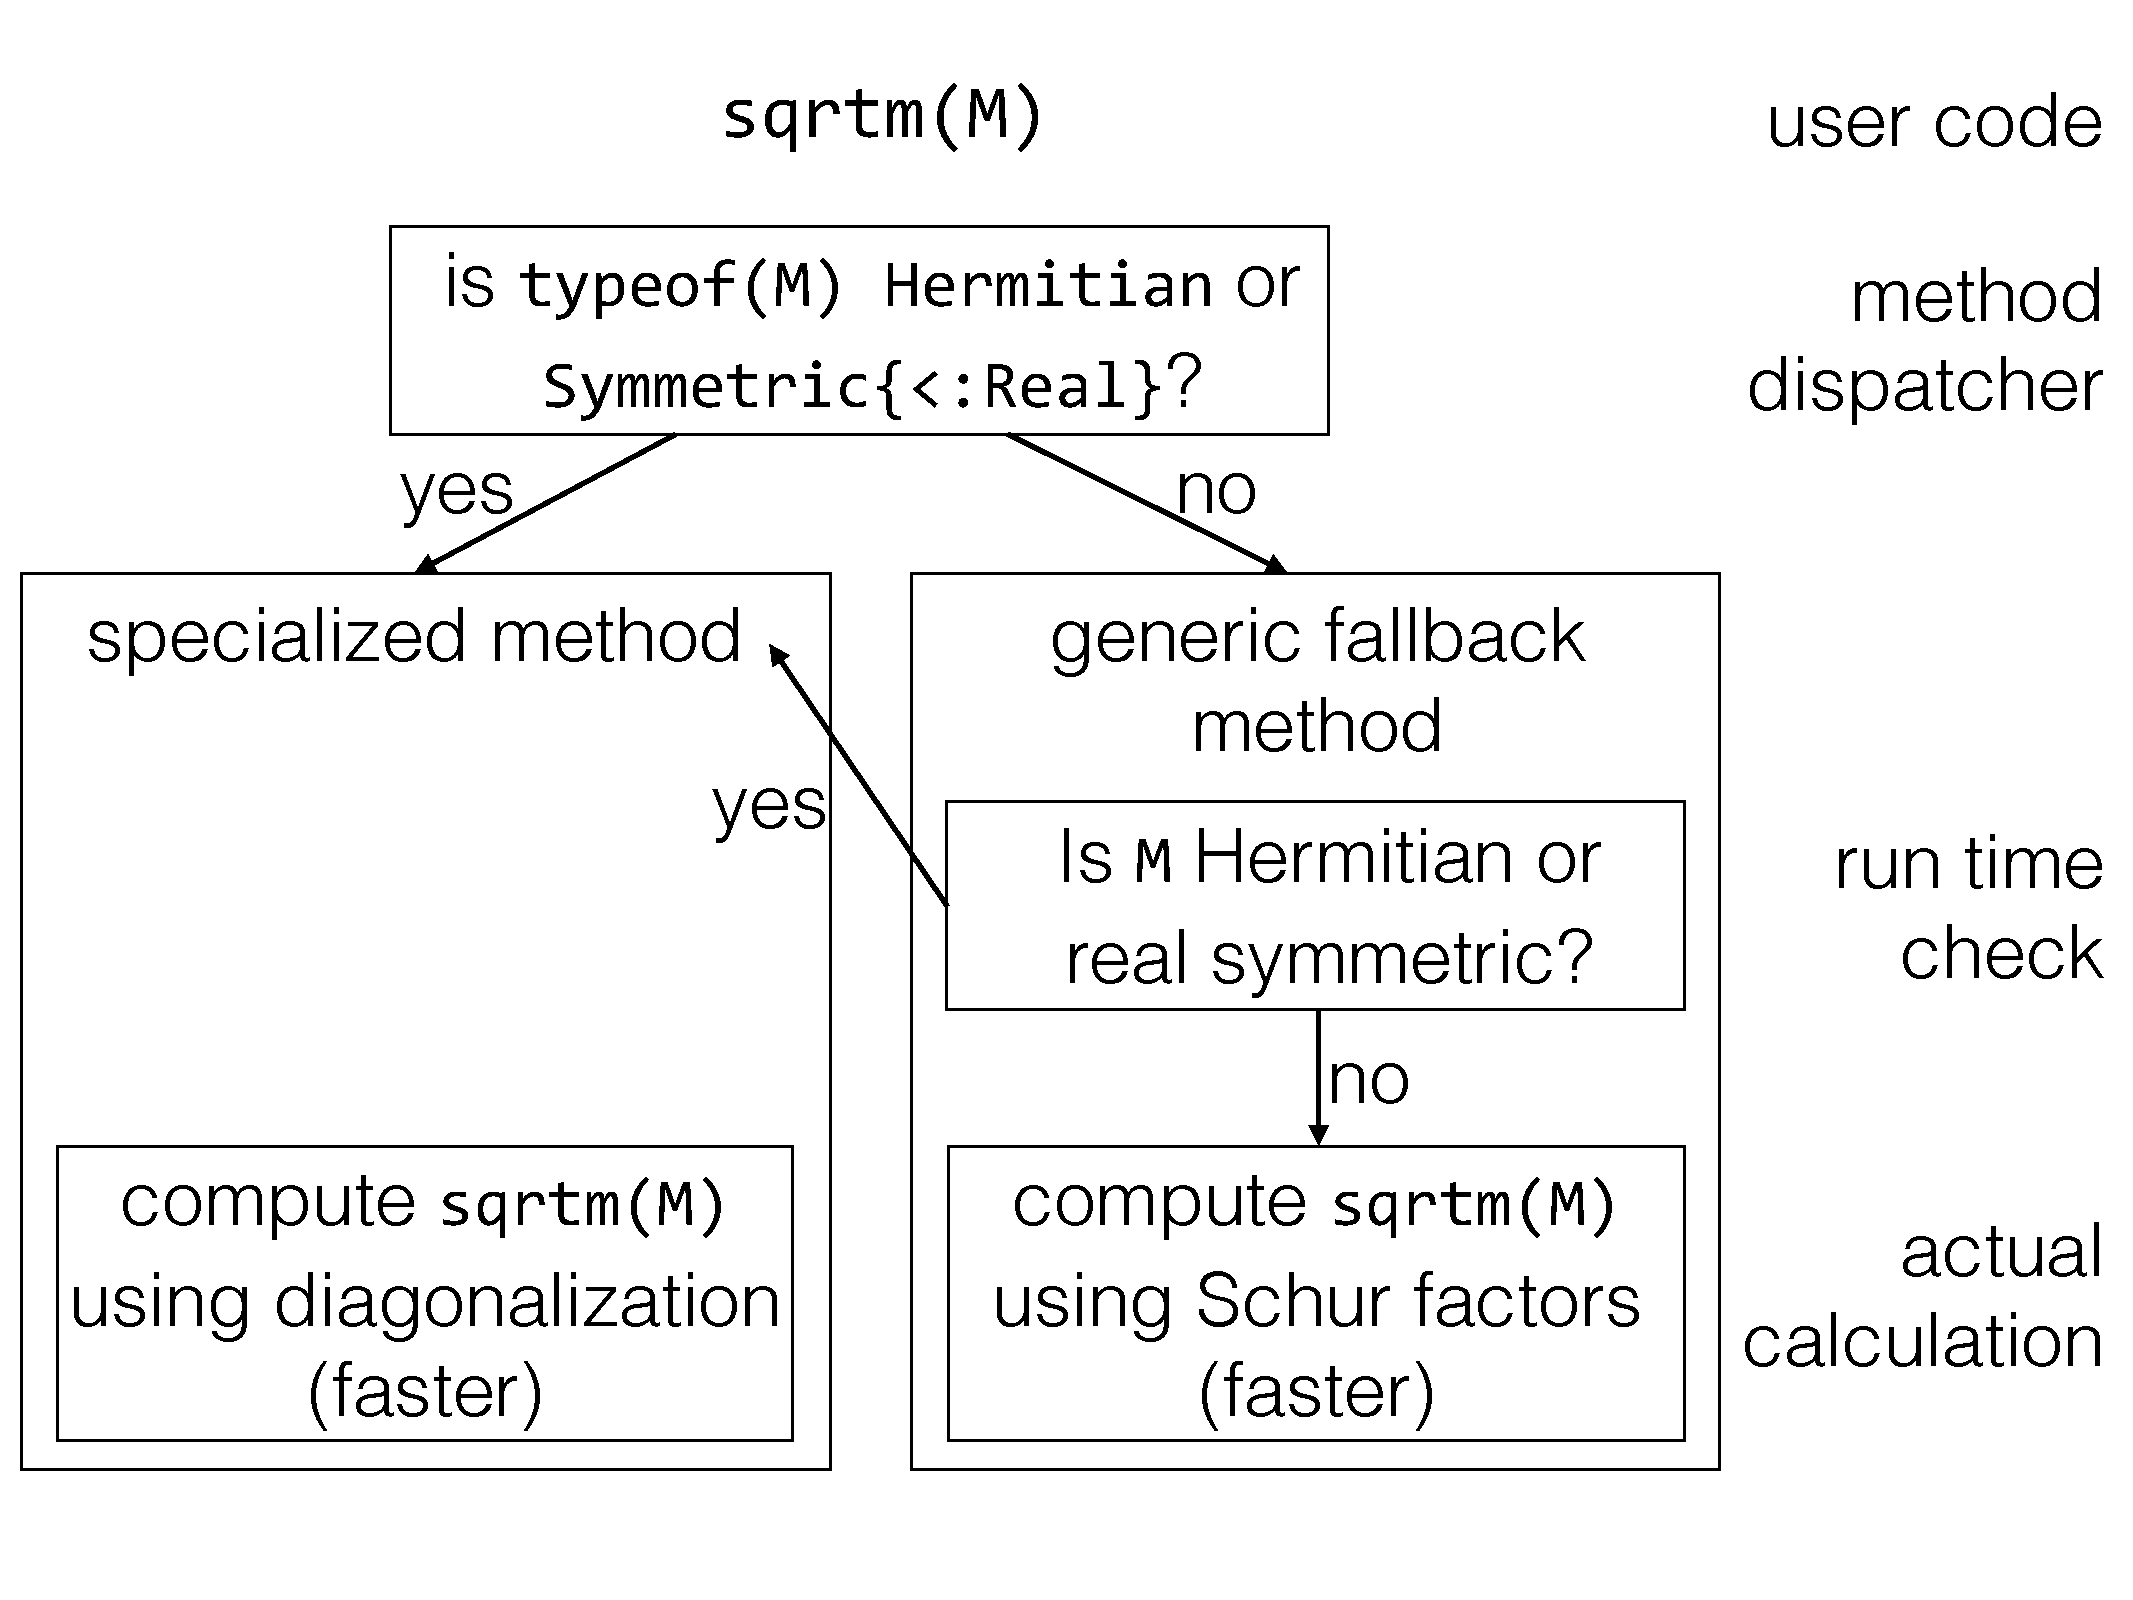
\includegraphics[width=\columnwidth]{fig-sqrtm}
	\caption{Dynamic dispatch and multimethods for the matrix square root
		function \texttt{sqrtm}, showing that the specialized algorithm
		can be run either from a static decision from the method
		dispatcher based on the input type, or a dynamic decision from
		a run--time check based on the value.}
	\label{fig:sqrtm}
\end{figure}

\subsection{Matrix factorization types}

Julia's base linear algebra library also provides extensive support for matrix
factorizations, which are indispensable for reasoning about the
interdependencies between matrices with special properties and the numerical
algorithms that they enable~\cite{Golub1996}. Many algorithms for numerical
linear algebra involve interconversions between general matrices and similar
matrices with special matrix symmetries. For many purposes, it is convenient to
reason about the resulting special matrix, together with the matrix performing
the transformation, as a single mathematical object rather than two separate
matrices. Such an object represents a matrix factorization, and is essentially
a different data structure that can represent the same content as a matrix
represented as an ordinary two--dimensional array.

The exact matrix factorization object relevant for a given linear algebra
problem depends on the symmetries of the starting matrix and also the
underlying field of matrix elements (i.e.\ whether the matrix contains real
numbers, complex numbers, or something else). In some use cases, these
properties may be known by the user as part of the problem specification, and
in other cases they may be unknown. Some properties, like whether a
matrix is triangular, can be deduced by inspecting the matrix elements for
$O(N^2)$ cost. Others, like whether a matrix is positive definite, require an
$O(N^3)$ computation in the general case, and is most efficiently determined by
attempting to compute the Cholesky factorization.

The resulting algorithm for determining a useful matrix factorization has to
capture the interplay between allowing the user to specify additional matrix
properties and attempting to automatically detect useful properties when the
additional cost of doing so is not prohibitive. The general case is implemented
in Julia's base library by the \verb|factorize| function, and typifies the
complexity associated with numerical codes: 

\begin{lstlisting}
function factorize{T}(A::Matrix{T})
    m, n = size(A)
    if m ==n #Is matrix square?
	#The factorization of a 1x1 matrix is just itself
        if m==1 return A[1] end
	
	#Is matrix upper triangular?
	utri = istriu(A)
	#Is matrix upper Hessenberg?
	utri1 = ishessenbergu(A)
	#Is matrix symmetric?
	sym = issym(A)
	#Is matrix Hermitian?
	herm = ishermitian(A)
	#Is matrix lower triangular
	ltri = istril(A)
	#Is matrix lower Hessenberg?
	ltri1 = ishessenbergl(A)
                    
	if ltri && utri
	    # A is both lower and upper triangular
	    # i.e. A is Diagonal
	    return Diagonal(A)
	elseif ltri && utri1
	    # A is lower triangular and upper Hessenberg
	    # i.e. A is upper Bidiagonal
	    return Bidiagonal(diag(A), diag(A, -1), false)
	elseif ltri
	    # A is is lower Triangular
	    return Triangular(A, :L)
	elseif ltri1 && utri
	    # A is lower Hessenberg and upper triangular
	    # i.e. A is lower bidiagonal
	    return Bidiagonal(diag(A), diag(A, 1), true)
	elseif ltri1 && utri1
	    # A is both lower and upper Hessenberg
	    # i.e. A is tridiagonal
	    if (herm && (T <: Complex)) || sym
	        # A is symmetric tridiagonal
		M = SymTridiagonal(diag(A), diag(A, -1))
		# _may_ be factorizable into
		# LDL' Cholesky form
		try
		    return ldltfact!(M)
                end
	    end
	    # A is tridiagonal
	    M = Tridiagonal(diag(A,-1), diag(A), diag(A,1))
	    # Factorize into tridiagonal LU form
	    return lufact!(M)
	elseif utri
	    # A is upper triangular
	    return Triangular(A, :U)
	elseif herm
	    # A is Hermitian
	    # _may_ be factorizable into Cholesky form
	    try
	        return cholfact(A)
	    end
	    # else use general Hermitian factorization
	    return factorize(Hermitian(A))
	elseif sym
	    # use general Symmetric factorization
	    return factorize(Symmetric(A))
	else # A is square but has no other symmetries
	    # Factorize into LU form
	    return lufact(A)
        end
    end #cases for square matrix A

    # A is rectangular
    
    # Can the result of a QR factorization be represented
    # using a floating point type supported by BLAS?
    const BlasFloat = Union(Float32, Float64, Complex64,
        Complex128)
    canuseBlasFloat = typeof(zero(T)/sqrt(zero(T) +
        zero(T)))<:BlasFloat)

    # Factorize into pivoted QR form where possible,
    # otherwise compute (unpivoted) QR form
    return qrfact(A, pivot=canuseBlasFloat)
end


# Factorize a Hermitian or Symmetric matrix into
# Bunch-Kaufman form as computed by bkfact
typealias HermOrSym Union(Hermitian, Symmetric)
factorize(A::HermOrSym) = bkfact(A.data, symbol(A.uplo),
    issym(A))
\end{lstlisting}

The \verb|factorize| function contains a few interesting features
designed to capture the highly dynamic nature of this computation:

\begin{enumerate}
\item The beginning checks for the ``easy'' properties, i.e.  those that can be
	computed cheaply at run--time by inspecting the matrix elements. The
	presence of one or more of these properties allow the input matrix
	\verb|A| to be classified into several special cases.

\item For many of these special cases (like \verb|Diagonal|), \verb|A| is
	explicitly converted to a special matrix type which allows dispatch on
	efficient specializations of linear algebraic operations that users may
	choose to perform later, such as matrix multiplication.
	
\item For other special cases (like \verb|Tridiagonal|), it is useful to
	attempt a run--time check for the ``hard'' properties, like positive
	definiteness, which require nontrivial computation. Computing the
	Cholesky factorization serves both as an efficient run--time check to
	detect positive definiteness, whose failure indicates lack thereof, and
	whose success yields a useful \verb|Cholesky| matrix factorization
	object which is useful for further computations such as solving linear
	equations or computing singular value decompositions (SVDs).

\item The \verb|Symmetric| and \verb|Hermitian| cases use control flow
	enabled by dynamic multimethods, as it is common for users to know
	whether the matrices they are working with have these properties.
	Using multimethods allows users to elide all the run--time checks
	in the generic method, skipping directly to the appropriate specialized
	method.

\item The base case contains a nontrivial runtime check to determine if the
	element type of \verb|A{T}| can be represented as a
	hardware--representable real or complex floating point number. The
	\verb|canuseBlasFloat| variable computes the type resulting from
	computations of the form $x / \sqrt{x + x}$, and checks that it is a
	subtype of \verb|BlasFloat|. The reason for this check is that there
	are two variants of the QR factorization: one pivoted, the other not.
	The former is generally preferred for numerical stability but is also
	significantly more difficult to compute, and hence is not yet
	implemented for all possible element types.

\end{enumerate}

In theory, it is possible to combine these structured matrix types under a
tagged union, e.g. in an ML-family language. However this would be
significantly less convenient. The problem is that in most contexts,
users are happy to have these objects separated by the type system, but
certain functions like \code{factorize} wish to combine them. It should be
possible to pass the result of such a function directly to an existing
routine that expects a particular matrix structure, without needing to
interpose case analysis to handle a tagged union.

It is also instructive to look more carefully at the methods for \verb|bkfact|,
which is but one of the several factorizations computed in \verb|factorize|:

\begin{lstlisting}
# Compute Bunch-Kaufman factorization,
# allocating new memory for the answer
bkfact{T<:BlasFloat}(A::StridedMatrix{T},
        uplo::Symbol=:U, symmetric::Bool=issym(A)) =
    bkfact!(copy(A), uplo, symmetric)

bkfact{T}(A::StridedMatrix{T}, uplo::Symbol=:U,
        symmetric::Bool=issym(A)) = bkfact!(convert(
    Matrix{promote_type(Float32,typeof(sqrt(one(T))))},A),
    uplo,symmetric)

# Compute Bunch-Kaufman factorization in-place

# For real symmetric matrices, call LAPACK SSYTRF or
# SSYTRF routine for T==Float32 or T==Float64 respectively
function bkfact!{T<:BlasReal}(A::StridedMatrix{T},
        uplo::Symbol=:U, symmetric::Bool=issym(A))
    symmetric || error("The Bunch-Kaufman decomposition
is only valid for symmetric matrices")
    LD, ipiv = LAPACK.sytrf!(char_uplo(uplo) , A)

    #Wrap answer in BunchKaufman type
    BunchKaufman(LD, ipiv, char_uplo(uplo), symmetric)
end

# For complex symmetric matrices, call LAPACK CSYTRF/ZSYTRF
# for T==Complex64/Complex128, and for complex Hermitian
# matrices, call the CHETRF/ZHETRF routines 
function bkfact!{T<:BlasComplex}(A::StridedMatrix{T},
	uplo::Symbol=:U, symmetric::Bool=issym(A))
    LD, ipiv = (symmetric ? LAPACK.sytrf! :
        LAPACK.hetrf!)(char_uplo(uplo) , A)
    BunchKaufman(LD, ipiv, char_uplo(uplo), symmetric)
end
\end{lstlisting}

The Bunch-Kaufman routines are implemented in two functions: \verb|bkfact|,
which allocates new memory for the answer, and \verb|bkfact!|, which mutates
the matrix in place to save memory. Reasoning about memory use is critical in
numerical linear algebra applications as the matrices may be very large.
Reusing allocated memory for matrices also avoids unnecessary copies of data to
be made, potentially minimizing memory accesses and reducing the need to
trigger garbage collection. The base library thus provides the latter for users
who need to reason about memory usage, and the former for users who do not.
Additionally, the type parameter \verb|T| describing the element type allows
for appropriate dispatch upon external LAPACK routines.


\subsection{Generic functions for statistical library routines}

Generic functions express a common action or computation, which may in
practice be performed in many different ways depending on the inputs. For
example, one may wish to compute the mean of a given statistical distribution.
In Julia, the computation can be expressed simply as dispatch onto the method
\code{mean(D::Distribution)}, with a different method for \code{mean} being
defined for different \code{Distribution}s. In contrast, much scientific code
is written in languages that lack generic functions, resulting in users having
to keep track of a large family of very closely related functions which
together can be thought of as specialized methods for a polymorphic function.
Table~\ref{statsfunctions} shows a family of closely related functions in the R
programming language and their Julia counterparts in the
\package{Distributions.jl} package. Julia provides a common functional interface
for each type of statistical distribution, with generic functions like
\code{pdf} to compute the probability density function, \code{cdf} for the
cumulative density function, \code{quantile} to compute quantiles, and
\code{rand} for sampling random variates. In contrast, each distribution in R
must have its own associated family of functions prefixed by \code{d},
\code{p}, \code{q} and \code{r} respectively, and the number of functions grows
by both the number of distributions and the number of desired computations on
them.

% \code{pdf}

\begin{table}
{\tiny
\begin{tabular}{l || l | l | l | l}
  \textbf{\code{D}}                & \textbf{\code{pdf(D)}}    & \textbf{\code{cdf(D)}}    &
        \textbf{\code{quantile(D)}} & \textbf{\code{rand(D)}}  \\ \hline\hline
  \textbf{\code{Beta}}             & \code{dbeta}     & \code{pbeta}     & \code{qbeta}       & \code{rbeta}    \\
  \textbf{\code{Binomial}}         & \code{dbinom}    & \code{pbinom}    & \code{qbinom}      & \code{rbinom}   \\
  \textbf{\code{Cauchy}}           & \code{dcauchy}   & \code{pcauchy}   & \code{qcauchy}     & \code{rcauchy}  \\
  \textbf{\code{Chisq}}            & \code{dchisq}    & \code{pchisq}    & \code{qchisq}      & \code{rchisq}   \\
  \textbf{\code{Exponential}}      & \code{dexp}      & \code{pexp}      & \code{qexp}        & \code{rexp}     \\
  \textbf{\code{Fdist}}            & \code{df}        & \code{pf}        & \code{qf}          & \code{rf}       \\
  \textbf{\code{Gamma}}            & \code{dgamma}    & \code{pgamma}    & \code{qgamma}      & \code{rgamma}   \\
  \textbf{\code{Geometric}}        & \code{dgeom}     & \code{pgeom}     & \code{qgeom}       & \code{rgeom}    \\
  \textbf{\code{Hypergeometric}}   & \code{dhyper}    & \code{phyper}    & \code{qhyper}      & \code{rhyper}   \\
  \textbf{\code{LogNormal}}        & \code{dlnorm}    & \code{plnorm}    & \code{qlnorm}      & \code{rlnorm}   \\
  \textbf{\code{Multinomial}}      & \code{dmultinom} & \code{pmultinom} & \code{qmultinom}   & \code{rmultinom}\\
  \textbf{\code{NegativeBinomial}} & \code{dnbinom}   & \code{pnbinom}   & \code{qnbinom}     & \code{rnbinom}  \\
  \textbf{\code{Normal}}           & \code{dnorm}     & \code{pnorm}     & \code{qnorm}       & \code{rnorm}    \\
  \textbf{\code{Poisson}}          & \code{dpois}     & \code{ppois}     & \code{qpois}       & \code{rpois}    \\
  \textbf{\code{TDist}}            & \code{dt}        & \code{pt}        & \code{qt}          & \code{rt}       \\
  \textbf{\code{Uniform}}          & \code{dunif}     & \code{punif}     & \code{qunif}       & \code{runif}    \\
  \textbf{\code{Weibull}}          & \code{dweibull}  & \code{pweibull}  & \code{qweibull}    & \code{rweibull} \\
\end{tabular}
}
\label{statsfunctions}
\caption{List of common distributions in R v3.1.1\cite{rlang} and their
associated functions. Shown in bold are the equivalent Julia generic
functions and \code{Distribution} types provided by the Julia package
\package{Distributions.jl}, showing how the namespace
is simplified by generic functions and multiple dispatch.}
\end{table}


\section{Evaluation}

Here we discuss the potential for performance in Julia's design,
as well as some shortcomings and challenges we have observed.

\subsection{Impact of static analyses on performance}

Figure~\ref{fig:timings} shows the relative execution times of benchmark codes
representing a wide variety of scientific applications, when various optimizations
and analyses are successively turned off. Relative to an unmodified Julia
distribution, first the LLVM optimization passes were turned off, followed by
some optimizations to elide allocation of tuples, function inlining, and finally
type inference. The results of type inference are used directly to perform
compile-time method lookup, while inference itself is only an analysis with
no performance effect. Therefore
we report on these technically-separate steps as a single item.
The relative
importances of each optimization pass were computed by taking ratios of
consecutive timings with and without that particular optimization pass.

On average, function inlining turned out to be the most important optimization
for improving the speed of Julia code, speeding up code by an average factor
19.93. Type inference came in second in importance at 6.89, followed by LLVM at
1.53. The allocation-elision optimization measured here turned
out to have almost no effect on execution speed, with an average contribution
of 0.99.

\begin{figure*}
	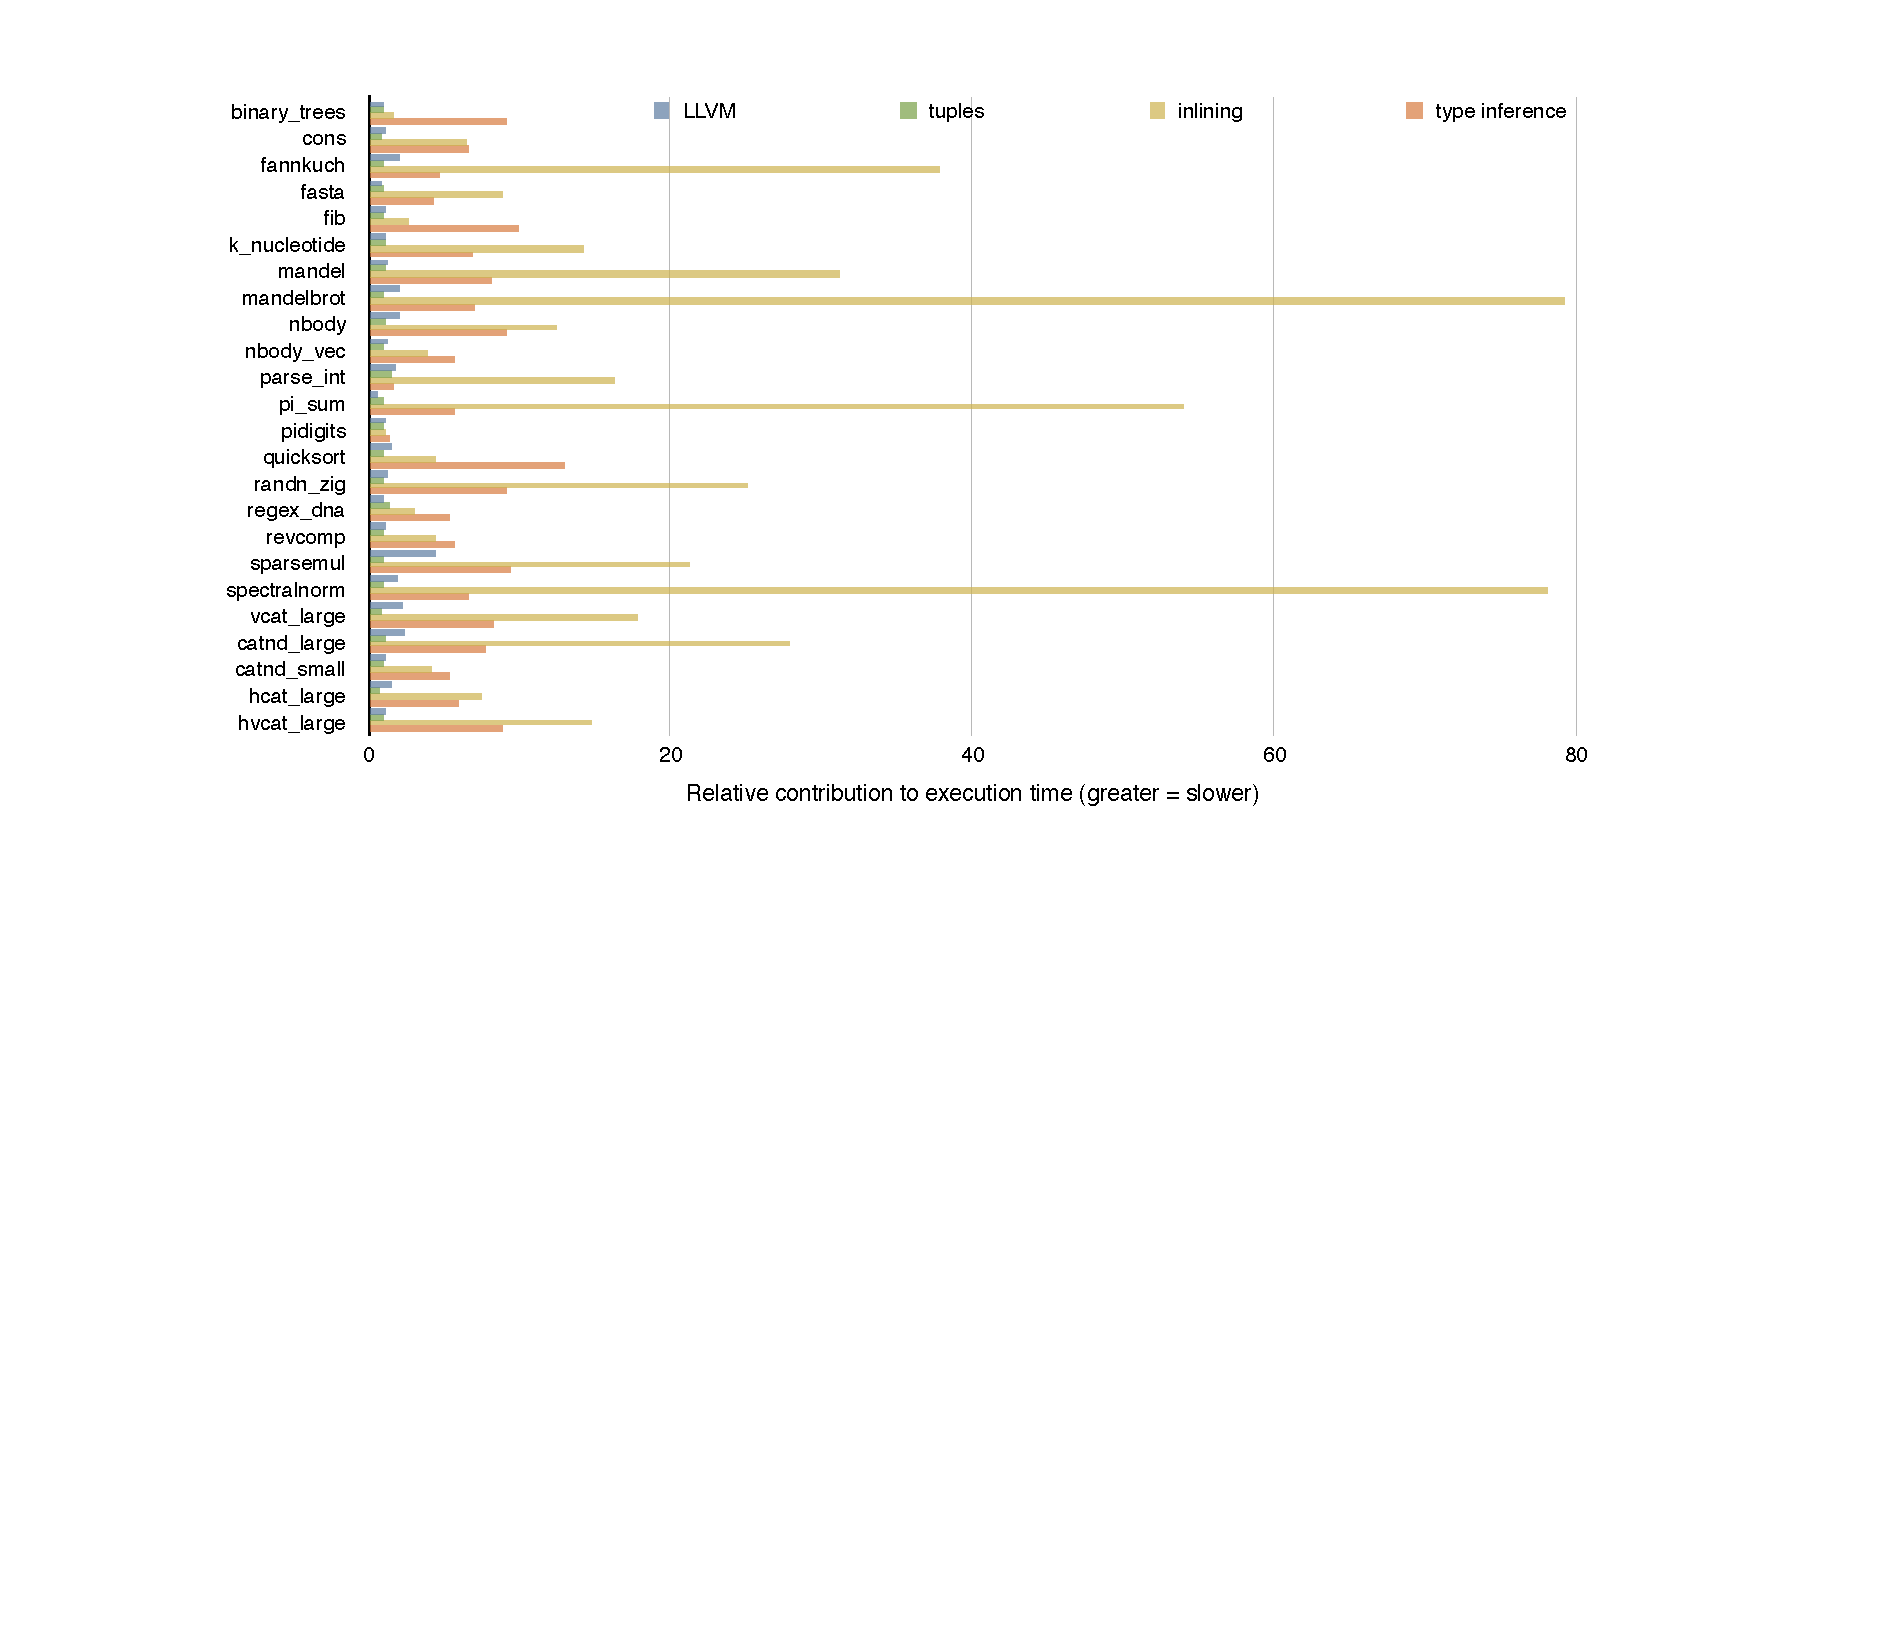
\includegraphics[width=\textwidth]{fig-timings}
	\caption{Relative contributions of various optimization passes to
	performance of Julia code implementing a representative collection
	of benchmarks. Bars from top to bottom represent: LLVM
	optimizations, tuple elision, function inlining, and type inference.}
	\label{fig:timings}
\end{figure*}


\subsection{Method ambiguities}

Julia uses symmetric multiple dispatch where all arguments have equal priority
for dispatch. This contrasts with some other languages like
Cecil~\cite{Chambers1992,Chambers1994} and Dylan~\cite{dylanman}, which
prioritize the arguments from left to right~\cite{Agrawal1991}. Julia instead
sorts methods by specificity~\cite{Bezanson2012}. For example, the function
\verb|f| defined by 

\begin{lstlisting}
f(x::Real, y::Int) = 1
f(x::Int, y::Real) = 2
\end{lstlisting}
%
results in a method ambiguity: because of subtype polymorphism, it is not clear
which method gets dispatched for inputs of type \verb|(Int, Int)|. To solve
this problem, Julia
requires a specialized method \verb|f(x::Int, y::Int)| to be defined before
these two methods.

Method ambiguity warnings were intended to reveal problems in multimethod
definitions. However, at other times it is a major nuisance for library
writers. The canonical example is trying to use \package{Images.jl} and
\package{DataFrames.jl} at the same time, which extend the \verb|AbstractArray|
type with additional subclasses in mutually incompatible ways. Adding an image
and a data frame is nonsensical and should return an error in client code that
attempts to do so. However, the method ambiguities are detected when a package
is loaded and compiled, throwing ambiguity warnings which may pertain to method
definitions that are never used. In practice, most user code avoids nonsensical
uses, but have other intentions in mind for using different functionality from
both packages in the same code. Nevertheless, the ambiguity warnings are
emitted even for code that avoids using the ambiguous methods in question.
Library writers are therefore faced with the unpleasant task of defining
disambiguating methods solely to suppress compile--time warnings, or otherwise
avoid the issue entirely by not using subtyping features of Julia, which could
reduce code reuse.

Work is underway to turn such method ambiguity warnings into run--time errors,
so that the responsibility of not running nonsensical methods is devolved onto
user client code, rather than burdening library writers with the need to
second--guess every conceivable corner case in the use of their libraries.

\subsection{Type stability}

New users migrating from other dynamic languages like MATLAB, Python and R are
often surprised that direct, line--for--line translations to Julia do not
achieve claimed C--like performance. Empirical reports~\cite{julia-users}
indicate that such users are unfamiliar with reasoning about types. One common
pitfall is \textbf{type instability}, which is exemplified in the following
code:

\begin{lstlisting}
function f()
   x = 0
   for y=1.0:1000000.0
      x += y
   end
end
\end{lstlisting}
%
This seemingly innocuous routine runs slowly because \verb|x| is initialized to
\verb|0| which is of type \verb|Int|, but accumulates floating point values
\verb|y| of type \verb|Float64| and so within the inner loop undergoes type
promotion to \verb|promote_type(Int,Float64)| \verb|== Float64|. The data flow
analysis thus cannot deduce that \verb|x| is a concrete type, but only that it
is of type \verb|Union(Int,| \verb|Float64)|. Thus the generated LLVM code must
call back to the Julia runtime to determine the value's actual type, and hence
boxes the value \verb|x|. As a result, \verb|x| cannot be mapped onto an LLVM
register, but must instead be heap allocated.

Another class of type instabilities results from the subtle interaction of
parametric invariance, the use of non-leaf type parameters and type promotion.
For example, the parametric type \verb|Complex{FloatingPoint}| is
type--unstable under addition (\verb|+|):

\begin{lstlisting}
function g()
    x = Complex{FloatingPoint}(1.0, 2.0f0) #(Float64, Float32)
    x + x #inferred type is Complex
end
\end{lstlisting}
%
Calling \verb|g()| returns a value of type \verb|Complex{Float64}| because the
\verb|+| method called uses the external constructor

\begin{lstlisting}
Complex(x::Real, y::Real) = Complex(promote(x,y)...)
\end{lstlisting}
%
which promotes the real and imaginary components to a common supertype (in this
case, \verb|Float64|). Since type parameters are invariant, the resulting type
is neither a subtype nor a supertype of the original type.

Most static languages like C require users to explicitly reason about type
instabilities (e.g.\ by requiring type casts); most dynamic languages allow
type--unstable code, but at the price of degraded performance. Julia allows
users to inspect the results of type inference and modify their codes to
improve performance by sharpening type annotations on variables, using language
constructs described in Section~\ref{sec:inference}.


\section{Related Work}

The more common programming languages that support dynamic multiple dispatch
are Cecil~\cite{Chambers1992,Chambers1994}, Common Lisp with
CLOS~\cite{Bobrow1988}, Clojure~\cite{Hickey2008} and Dylan~\cite{dylanman}.
These languages also differ in the dispatch rules: Cecil, like Julia, employs
symmetric multiple dispatch; CLOS and Dylan resolve ambiguities by matching
arguments from leftmost to rightmost, and Clojure's dispatch rules are
customizable based on user--specifiable rules. The method dispatchers are also
limited in their expressiveness by the type system of their host languages.
Clojure's multimethods are not a core language construct and hence interact
only weakly with built--in types. Dispatch in CLOS is class--based and excludes
parametric types. Cecil's type system supports subtype polymorphism but not
type parameters. Dylan supports CLOS--style class--based dispatch, and also
let--polymorphism in limited types, which is a restricted form of parametric
polymorphism. However, Dylan does allows for multiple inheritance.



%% \section{Implementation challenges}

%% Julia allows technical computing users to write expressive, performant code
%% that makes use of advanced language constructs. However, users sometimes still
%% face challenges in writing code that expresses what they want. This section
%% gives some examples of problems faced by Julia users and how the language is
%% still evolving to address the needs of users and improve their overall user
%% experience.

%% JWB: I think this section is really not interesting and not related to
%% multiple dispatch enough.

%% \subsection{(Data) vectorization}

%% New Julia users are also often surprised that vectorized expressions in Julia
%% can be slower than their devectorized counterparts. Consider the function

%% \begin{lstlisting}
%% h1(x) = sin(x) + im*cos(x)
%% \end{lstlisting}
%% %
%% For scalar numbers \verb|x| of type \verb|Float64|, \verb|h1| constructs a
%% complex number of type \verb|Complex{Float64}|. However, \verb|h1| also accepts
%% arrays of type \verb|Array{Float64, N}| (where $N$ is the rank), returning a
%% corresponding array \verb|Array{Complex| \verb|{Float64}, N}|.

%% In other dynamic languages, vectorization is an accepted mantra for
%% performance~\cite{matlabuserguide,Langtangen2008}, as the vectorized functions often wrap
%% kernels written in a low--level language that deliver performance over
%% functionally equivalent devectorized code which use slow, directly interpreted
%% scalar loops~\cite{Seljebotn2009,Walt2011}. Users have therefore learned that
%% vectorized functions provide speed, and will sometimes go to great lengths to
%% contort their computations into vectorized form to speed up their code, even if
%% the computation cannot be expressed conveniently or naturally in vectorized
%% form. Furthermore, vectorization still incurs significant overhead,
%% particularly in the unwanted allocation of array temporaries. In this example,
%% \verb|h1| constructs three temporary arrays on top of the new array needed to
%% contain the answer, namely the arrays \verb|A|, \verb|B| and \verb|C| in the
%% equivalent code: 

%% \begin{lstlisting}
%% function h2(x)
%%     A = sin(x) #Apply sin to each element of x, etc.
%%     B = cos(x)
%%     C = im * B
%%     D = A + C
%%     return D
%% end
%% \end{lstlisting}
%% %
%% In contrast, the devectorized version of the same code

%% \begin{lstlisting}
%% function h3(x)
%%     z = similar(x) #Construct array with same shape as x
%%     for (i, y) in enumerate(x)
%%         z[i] = sin(y) + im*cos(y)
%%     end
%% end
%% \end{lstlisting}
%% %
%% computes the same result but avoids allocating temporary arrays and their
%% concomitant overhead costs for heap allocation, memory access and garbage
%% collection. Thus devectorized code is preferred in Julia as scalar loops are
%% fast with minimal overhead~\cite{Bezanson2014b}. 

%% \subsection{Vectorization and higher--order functions}

%% Users familiar with other dynamic languages for technical computing are used to
%% working with vectorized functions~\cite{matlabuserguide,Langtangen2008}:
%% \verb|sin(x)| should work on both scalar and vector arguments \verb|x|. However,
%% vectorized functions have limited
%% extensibility and composability. Implementations can only bless some
%% functions to be vectorized; vectorized functions which wrap external low--level
%% kernels lack code reuse and cannot be extended easily. In contrast, the Julia
%% standard library implements vectorized functions consistently using using code
%% generated by the macros \verb|@vectorize_1arg|, \\
%% \verb|@vectorize_2arg|, etc.

%% The composability problem is more subtle. The generic function \verb|h1| has
%% methods with function types

%% \begin{itemize}
%% 	\item \verb|Float64| $\rightarrow$ \verb|Complex{Float64}|,
%% 	\item \verb|Vector{Float64}| $\rightarrow$ \verb|Vector{Complex{Float64}}|,
%% \end{itemize}
%% %
%% and others, and writing a function \verb|i(x)| that composes properly with
%% \verb|h1| must account for all possible outputs of the latter, be they scalars
%% or arrays. Thus \verb|i(x)| must also be vectorized, but the dynamic nature of
%% Julia precludes any restrictions on the methods that must be defined for
%% \verb|i|, placing the burden of correct implementation on users and library
%% writers.

%% The example of \verb|h1| suggests that what users really want is not vectorized
%% functions, but rather convenient syntax for vectorized \textit{expressions}.
%% The \package{Devectorize.jl} package uses code generation techniques to marry
%% the convenient syntax for vectorized functions with the speed of devectorized
%% code with explicit loops. The restructuring for vectorization is often
%% unnatural, and at times not possible. Alternatively, a more general approach is
%% to use higher order functions like \verb|map| to compute an entire vectorized
%% expression, like so:

%% \begin{lstlisting}
%% h3(x) = map(_ -> sin(_) + im*cos(_), x)
%% \end{lstlisting}
%% %
%% \verb|map| provides an elegant solution to mapping a computation over a
%% collection of input data. However, implementing \verb|map| efficiently in Julia
%% touches upon all the aspects of the type system, generic function system,
%% dispatch, and type inference that have been discussed above:

%% \begin{enumerate}

%% 	\item The output type of \verb|f| must be an \verb|Array{T}| with
%% 	element type \verb|T| wide enough to describe all the possible output
%% 	elements. \verb|T = Any| is the widest possible array, but provides no
%% 	information about the mutability of each element. Consequently the
%% 	array must be represented in memory with pointers to boxed elements. In
%% 	contrast, being able to infer a concrete immutable element type like
%% 	\verb|T = Float64| allows the indirection to array elements and the
%% 	overhead of tagging to be eliminated, allowing the resulting array data
%% 	to stored contiguously like a C or Fortran array.

%% 	\item To know the output type of \verb|f(y)| for some element \verb|y|
%% 	of \verb|x|, the type of \verb|y| must be known so that the actual
%% 	method being dispatched for the generic function \verb|f| can be looked
%% 	up in the dispatch table. This means that the data \verb|x| must be
%% 	fully typed within the type environment where \verb|map| is invoked.
%% 	Furthermore the type environment must yield enough information about
%% 	\verb|y| so that the method dispatcher is able to pick out a
%% 	specialized method over the generic fall--back for \verb|f|.

%% 	\item Since Julia lacks true function types, the output type of
%% 	\verb|f(y)| must be inferred from data flow analysis, and the inferred
%% 	type must be sufficiently sharp to determine the type of the output of
%% 	\verb|map|.

%% 	\item For performance, the scalar operation \verb|f(y)| must be
%% 	inlined, and hence the inlining code transformation pass must deem the
%% 	inlining to be viable.

%% 	\item Implementing \verb|map| over an arbitrary iterable \verb|x| is
%% 	harder than implementing vectorized functions, since the former lacks
%% 	the guarantee provided by \verb|Array| inputs types that every element
%% 	has the same type. In the worst case, the method dispatcher must be
%% 	called for each element \verb|y| just to find out which method is
%% 	dispatched for \verb|f(y)|.

%% \end{enumerate}

%% The implementation of \verb|map| hence speaks to the conflicting demands of
%% flexibility and performance that underlie the design tradeoffs built into
%% Julia's types, generic functions and type inference algorithms. The current
%% implementation leverages empirical evidence that most applications use
%% homogeneous arrays of concrete types, and most other applications have
%% heterogeneity that be detected early on~\cite{Bolz2013}. Hence, \verb|map|
%% optimistically assumes an element type based on the output returned from the
%% first element, and makes further copies into increasingly wider arrays as
%% necessary if a later return type is wider than the current element type. The
%% number of such copies made is bounded by the maximal height of the type
%% lattice, and the aggressive method specialization in Julia's compiler can emit
%% specialized code which optimize away branch checks for widening in cases where
%% the input type is completely known, e.g.\ when the input is an \verb|Array|
%% with some concrete element type, and thus avoid the cost of conditional
%% branches.

\section{Conclusion}

Julia as a language is still evolving, and there is room for further
improvements to the compiler, such as additional static analyses for peephole
optimizations, constant propagation, and backward data flow type inference.
Nevertheless, the current type system, generic function system with
multimethods and type inference with aggressive method specialization afford
rich semantics which are useful for technical computing applications.
Furthermore, the design and interaction between these language components allow
users to design their own Pareto--optimal tradeoffs between performant
specialization and flexible generality within a single programming language.




\acks{We thank the many Julia users and developers for their contributions to
the Julia language.}

%The authors gratefully acknowledge support from the MIT Deshpande center for
%technical innovation, the Intel Technology Science Center for Big Data, the
%DARPA XDATA program, the Singapore--MIT Alliance, NSF Awards CCF-0832997 and
%DMS-1016125, VMWare Research, a DOE grant with Dr. Andrew Gelman of Columbia
%University for petascale hierarchical modeling, a Citibank grant for High
%Performance Banking Data Analysis, and the Levine Fellowship.}

\bibliographystyle{abbrvnat}
\bibliography{pldi2015,websites}

\end{document}
